\documentclass[10pt,a4paper]{article}
\usepackage[utf8]{inputenc}
\usepackage[a4paper,%
            left=.75in,right=.75in,top=1in,bottom=1in]{geometry}
\setlength{\headsep}{0.25in}

\usepackage{amsthm}

\usepackage{graphicx}
\usepackage{pgfplots}
            
\usepackage[english]{babel}

\theoremstyle{theorem}
\newtheorem{theorem}{Theorem}
\newtheorem{lemma}{Lemma}
\newtheorem{corollary}{Corollary}
\newtheorem{case}{Case}

\usepackage{listings}
\usepackage{color} %red, green, blue, yellow, cyan, magenta, black, white
\definecolor{mygreen}{RGB}{28,172,0} % color values Red, Green, Blue
\definecolor{mylilas}{RGB}{170,55,241}

\newcommand\restr[2]{{% we make the whole thing an ordinary symbol
  \left.\kern-\nulldelimiterspace % automatically resize the bar with \right
  #1 % the function
  \vphantom{\big|} % pretend it's a little taller at normal size
  \right|_{#2} % this is the delimiter
  }}

\theoremstyle{definition}
\newtheorem{definition}{Definition}
\newtheorem{remark}{Remark}

\usepackage{mathtools}
\DeclarePairedDelimiter\bra{\langle}{\rvert}
\DeclarePairedDelimiter\ket{\lvert}{\rangle}
\DeclarePairedDelimiterX\braket[2]{\langle}{\rangle}{#1 \delimsize\vert #2}

\usepackage{amsmath}
\usepackage{amsfonts}
\usepackage{amssymb}
\usepackage{fancyhdr}

\DeclareMathOperator{\interior}{int}

\newcommand{\Tau}{\mathcal{T}}

\newenvironment{amatrix}[1]{%
  \left(\begin{array}{@{}*{#1}{c}|c@{}}
}{%
  \end{array}\right)
}

\usepackage{calligra}
\DeclareMathAlphabet{\mathcalligra}{T1}{calligra}{m}{n}
\DeclareFontShape{T1}{calligra}{m}{n}{<->s*[2.2]callig15}{}

\newcommand{\scripty}[1]{\ensuremath{\mathcalligra{#1}}}

\pagestyle{fancy}
\author{Jeremiah Givens}
\newcommand{\subject}{Metric Spaces}
\newcommand{\Date}{9/2/2021} 
\makeatletter
\rhead{{\small\@author}}
\lhead{{\small\subject}}
\chead{{\large Picard's Existence and Uniqueness Theorem}}
\cfoot{}
\rfoot{\thepage}
\lfoot{\today}

\renewcommand{\theequation}{\arabic{equation}}

\begin{document}

\lstset{language=Matlab,%
    %basicstyle=\color{red},
    breaklines=true,%
    morekeywords={matlab2tikz},
    keywordstyle=\color{blue},%
    morekeywords=[2]{1}, keywordstyle=[2]{\color{black}},
    identifierstyle=\color{black},%
    stringstyle=\color{mylilas},
    commentstyle=\color{mygreen},%
    showstringspaces=false,%without this there will be a symbol in the places where there is a space
    numbers=left,%
    numberstyle={\tiny \color{black}},% size of the numbers
    numbersep=9pt, % this defines how far the numbers are from the text
    emph=[1]{for,end,break},emphstyle=[1]\color{red}, %some words to emphasise
    %emph=[2]{word1,word2}, emphstyle=[2]{style},    
}

\begin{titlepage}
\vspace*{\fill}
\begin{center}
{\Huge Picard's Existence and Uniqueness Theorem}\\
Author: Jeremiah Givens\\
Professor: Dr. Claudio Morales\\
Deparment of Mathematics, University of Alabama in Huntsville
\end{center}
\vspace*{\fill}
\end{titlepage}

\section{Introduction}
The main objective of this paper is to examine a very practical application of Banach's fixed point theorem: Picard's Existence and Uniqueness Theorem for Ordinary Differential Equations. We will begin by proving some useful lemmas, which we will then use to prove Picard's theorem. After proving the theorem, we will then look at a few example differential equations that Picards theorem proves the existence of solutions to, and we will use an iterative technique, known as the Picard Iteration, to approximate the solutions.

\section{Preliminaries}
\begin{lemma}
Let $x: [a, b] \to \mathbb{R}$ be continuous. Then, $x$ is bounded, and $x$ achieves it's maximum.
\end{lemma}

\begin{proof}
We have
\begin{align*}
[a, b] \text{ is compact} &\implies x([a, b]) \text{ is compact} && \text{continuous image of compact set}\\
&\implies x([a, b]) \text{ is closed and bounded} && \text{by the Heine-Borel Theorem, since } x([a, b]) \subseteq \mathbb{R}\\
&\implies x \text{ is bounded}.
\end{align*}

Now we need to show that $x$ achieves its maximum.  We know from our argument above, that $x$ has an upper bound. Thus, the least upper bound property of the real numbers tells us that the supremum $M = \sup \{x(t): t \in [a, b] \}$ exists. By the definition of a supremum, we can choose a sequence $\{t_n \}_{n \in \mathbb{N}}$ such that $M- \frac{1}{n} \leq x(t_n) \leq M$. Clearly, the sequence $\{x(t_n)\}_{n \in \mathbb{N}}$ converges to $M$. Since $[a, b]$ is compact, and therefore sequentially compact, we have that $\{t_n \}_{n \in \mathbb{N}}$ has a subsequence $\{t_{n_i} \}_{i \in \mathbb{N}}$ that converges to some $t \in [a, b]$. Since $x$ is continuous, $\{x(t_{n_i}) \}_{i \in \mathbb{N}}$ converges to $x(t)$. Since a subsequence of any convergent sequence converges to the same limit, we have that $\{x(t_{n_i}) \}_{i \in \mathbb{N}}$ converges to $M$. Therefore,  $x$ achieves its maximum at $t$.
\end{proof}

\begin{lemma}
Let $C$ equal the set of all continuous real-valued functions on the closed interval $[a, b]$. Then, $C$ forms a metric space with the metric $d$ defined by
\begin{align*}
d(x, y) = \max_{t \in [a, b]} |x(t) - y(t)|.
\end{align*}
\end{lemma}

\begin{proof}
Since we know every norm induces a metric, it will suffice to show that $|| \cdot ||: C \to \mathbb{R}$ defined by
\begin{align*}
||x|| = \max_{t \in [a, b]} |x(t)|
\end{align*}
forms a norm on $C$. Since the absolute value function is continuous, and the composition of two continuous functions is continuous, we can conclude from Lemma 1 that $|| x ||$ is well defined for all $x \in C$.

Let $s \in \mathbb{R}$, and $x \in C$. We have
\begin{align*}
||s x|| &= \max_{t \in [a, b]} |s x(t)|\\
&= \max_{t \in [a, b]} |s|| x(t)|\\
&= |s|\max_{t \in [a, b]} | x(t)| && \text{since } s \text{ has no dependence on } t\\
&= |s|||x||,
\end{align*}
and we have shown that $|| \cdot ||$ obeys the absolute homogeneity property of a norm.

Next, we must show that for all $x \in C$, $||x|| = 0 \implies x = 0$. Let $x \in C$. Proving the contrapositive, we have 
\begin{align*}
x \not = 0 &\implies (\exists t_0 \in [a, b])(x(t_0) \not = 0)\\
&\implies \max_{t \in [a, b]} |x(t)| \geq |x(t_0)| && \text{by definition of a max}\\
&\implies \max_{t \in [a, b]} |x(t)| > 0\\
&\implies ||x|| > 0.
\end{align*}

Finally, we must show that the triangle inequality holds for $|| \cdot ||$. Let $x, y \in C$. By Lemma 1, we have that $|x|$, $|y|, $ and $|x + y|$ achieve their maximums on $[a, b]$. Thus, we can define $t_1,t_2,t_3 \in [a, b]$ to be such that $|x(t_1)| = ||x||$, $|y(t_2)| = ||y||$, and $|x(t_3) + y(t_3)| = ||x + y||$. With this, we have
\begin{align*}
||x + y|| &= |x(t_3) + y(t_3)|\\
&\leq |x(t_3)| + |y(t_3)| && \text{Since the absolute value function forms a norm on the real numbers}\\
&\leq |x(t_1)| + |y(t_3)| && \text{Since } |x(t_1)| \geq |x(t_3)| \text{ by definition of a max}\\
&\leq |x(t_1)| + |y(t_2)| && \text{Since } |y(t_2)| \geq |y(t_3)| \text{ by definition of a max}\\
&= ||x|| + ||y||,
\end{align*}
and our proof is complete.
\end{proof}

\begin{lemma}
The metric space $(C, d)$ from the previous lemma is complete.
\end{lemma}

\begin{proof}
Let $\{x_n\}_{n \in \mathbb{N}}$ be a Cauchy sequence in $C$.  Define $f:[a, b] \to \mathbb{R}$ by $f(t) = \lim_{n \to \infty} x_n(t)$. We need to show that $f$ is well defined, that $f$ is continuous, and that $f = \lim_{n \to \infty} x_n$.

To show that $f$ is well defined, it will suffice to show that for all $t \in [a, b]$, the sequence $\{x_n(t) \}_{n=1}^\infty$ is Cauchy, since $\mathbb{R}$ is complete. Let $\epsilon > 0$. Since $\{x_n\}_{n \in \mathbb{N}}$ is Cauchy, there exists an $N \in \mathbb{N}$ such that for all $n, m \geq N$,
\begin{align*}
||x_n - x_m|| < \epsilon &\iff \max_{t \in [a, b]} |x_n(t) - x_m(t)| < \epsilon\\
&\implies (\forall t \in [a, b])(|x_n(t) - x_m(t)| < \epsilon).
\end{align*}
From this, we can conclude that $f$ is well defined.

We will now show that $f$ is continuous. Let $\epsilon >0$, and let $p_0 \in [a, b]$. Since $\{x_n(p)\}_{n \in \mathbb{N}}$ converges to $f(p)$ for all $p \in [a, b]$, there exists an $n \in \mathbb{N}$ such that $|f(p) - x_{n}(p)| < \frac{\epsilon}{3}$. Since $x_n$ is continuous at $p_0$, there exists a $\delta > 0$ such that for all $p \in [a, b]$
\begin{align*}
|p - p_0| < \delta \implies |x_n(p) - x_n(p_0)| < \frac{\epsilon}{3}.
\end{align*} 
With this, we have that for all $p \in [a, b]$ with $|p - p_0| < \delta$
\begin{align*}
|f(p) - f(p_0)| &\leq |f(p) - x_{n}(p)| + |f(p_0) - x_{n}(p)| &&\text{triangle inequality}\\
&\leq |f(p) - x_{n}(p)| + |f(p_0) - x_{n}(p_0)| + |x_n(p_0) - x_{n}(p)| &&\text{triangle inequality} \\
&< \frac{\epsilon}{3} + \frac{\epsilon}{3} + \frac{\epsilon}{3}\\
&= \epsilon.
\end{align*}
Thus, we have that $f$ is continuous, and therefore $f \in C$.

Finally, all that remains is to show that $f = \lim_{n \to \infty} x_n$. Let $\epsilon >0$. Since $\{x_n(p)\}_{n \in \mathbb{N}}$ is Cauchy, there exists an $N \in \mathbb{N}$ such that for all $m, n \geq N$, we have $||x_n - x_m|| < \epsilon$. Then, for all $t \in [a, b]$ and $m \geq N$, we have
\begin{align*}
|f(t) - x_m(t)| &= |\lim_{n \to \infty} x_n(t) - x_m(t)| && \text{by definition of } f\\
&= \lim_{n \to \infty}|x_n(t) - x_m(t)| && \text{by elemetary limit laws}\\
&\leq \lim_{n \to \infty}||x_n - x_m|| && \text{by definition of our norm}\\
&\leq \epsilon. && \text{by definition of } N \text{ above}
\end{align*}
Thus, since $\epsilon$ was arbitrary, we have shown that $f = \lim_{n \to \infty} x_n$, and that $C$ is complete.
\end{proof}

\begin{lemma}
Let $x_0 \in \mathbb{R}$, and let $c \in (0, \infty)$. Let $\tilde{C}$ be a subspace of the metric space from Lemma 1, consisting of all functions $x \in C$ such that 
\begin{align*}
d(x, x_0) \leq c.
\end{align*}
Then, $\tilde{C}$ is closed.
\end{lemma}

\begin{proof}
Let $f \in \bar{\tilde{C}}$.  We have
\begin{align*}
f \in \bar{\tilde{C}} &\iff (\forall \epsilon > 0)(B(f; \epsilon) \cap \tilde{C} \not = \emptyset)\\
&\iff (\forall \epsilon > 0)(\exists x \in \tilde{C})(d(f, x) < \epsilon)\\
&\iff (\forall n \in \mathbb{N})(\exists x_n \in \tilde{C})(d(f, x_n) < \frac{1}{n}).
\end{align*}
With this, we have
\begin{align*}
d(f, x_0) &\leq d(f, x_n) + d(x_n, x_0) && \text{triangle inequality}\\
&< \frac{1}{n} + d(x_n, x_0)\\
&\leq \frac{1}{n} + c && \text{since } x_n \in \tilde{C}\\
\end{align*}
Since this is true for all $n \in \mathbb{N}$, we have $d(f, x_0) \leq c$ which implies $f \in \tilde{C}$.
\end{proof}

\begin{lemma}
Let $C$ be a complete metric space. Let $A \subseteq C$ be closed. Then, $A$ is complete.
\end{lemma}

\begin{proof}
Let $A$ be closed, and let $\{x_n\}_{n \in \mathbb{N}}$ be a Cauchy sequence in $A$.  Since $X$ is complete, we know that the limit converges to some point $x$ in $X$.  We have
\begin{align*}
\lim_{n \to \infty} x_n = x &\implies (\forall \epsilon > 0)(\exists N \in \mathbb{N})(n \geq N \implies d(x_n, x) \leq \epsilon)\\
&\implies (\forall \epsilon > 0)(\exists x_n \in A)(x_n \in B(x; \epsilon))\\
&\implies (\forall \epsilon > 0)(B(x; \epsilon) \cap A \not = \emptyset)\\
&\implies x \in \bar{A}\\
&\implies x \in A. && \text{since } A \text{ is closed}
\end{align*}
Since this is true for any Cauchy sequence in $A$, $A$ is complete.
\end{proof}

\section{Main Topic}
The focus of this paper is on solutions to explicit ordinary differential equation initial value problems of the form
\begin{align}
x' = f(t, x) \text{ with initial condition } x(t_0) = x_0,
\end{align}
where $x: \mathbb{R} \to \mathbb{R}$, $f: \mathbb{R} \times \mathbb{R} \to \mathbb{R}$, and the prime denotes differentiation of $x$ with respect to $t$.

\begin{theorem}
Let $f$ be continuous on a rectangle 
\begin{align*}
R = \{(t, x) \mathbb \in {R}^2 : |t - t_0| \leq a \land |x - x_0| \leq b \},
\end{align*}
and thus bounded on $R$, say
\begin{align}
|f(t, x)| \leq c, \text{ for all } (t, x) \in R.
\end{align}
Suppose $f$ satisfies a Lipschitz condition on $R$ with respect to it's second argument, that is, there is a constant $k$ (Lipschitz constant) such that for $(t, x), (t, v) \in R$
\begin{align}
|f(t, x) - f(t, v)| \leq k |x - v|.
\end{align}
Then the initial value problem (1) has a unique solution. This solution exists on an interval $[t_0 - \beta, t_0 + \beta]$ where 
\begin{align}
\beta < \min \Bigg \{a, \frac{b}{c}, \frac{1}{k} \Bigg \}
\end{align}
\end{theorem}

\begin{proof}
Let $C(J)$ be the metric space of all real-valued continuous functions on the interval $J = [t_0 - \beta, t_0 + \beta]$ with metric $d$ defined by 
\begin{align*}
d(x, y) = \max_{t \in J} |x(t) - y(t)|.
\end{align*}
By Lemma 2 we know that $C(J)$ is a metric space, and by Lemma 3 we know that $C(J)$ is complete.  Let $\tilde{C}$ be a subspace of $C(J)$ consisting of all functions $x \in C(J)$ such that 
\begin{align}
|x(t) - x_0| \leq c \beta.
\end{align}
By Lemma 4,  we have that $\tilde{C}$ is closed, so by Lemma 5 $\tilde{C}$ is complete.

From the fundamental theorem of calculus, (1) can be written in the form $x = Tx$, where $T: \tilde{C} \to \tilde{C}$ is defined by 
\begin{align}
Tx(t) = x_0 + \int_{t_0}^{t} f(\tau, x(\tau))d \tau
\end{align}
We have $\tau \in J \implies |\tau - t_0| \leq a$ (by 4), and 
\begin{align*}
x \in \tilde{C} &\implies |x(\tau) - x_0| \leq c \beta &&\text{by (5)}\\
&\implies |x(\tau) - x_0| \leq b &&\text{by (4)}.
\end{align*}
Thus, $(\tau, x(\tau)) \in R$ and the integral in (6) exists since $f$ is continuous on $R$.We must show that $Tx$ is continuous, and that $T$ maps $\tilde{C}$ into itself. To see that $Tx$ is continuous, let $\epsilon >0$. We have, for any $t_1, t_2 \in J$, with $t_1 \geq t_2$, we have
\begin{align*}
|Tx(t_1) - Tx(t_2)| &= \left| x_0 + \int_{t_0}^{t_1} f(\tau, x(\tau))d \tau - x_0 - \int_{t_0}^{t_2} f(\tau, x(\tau))d \tau\Large\right|\\
&= \left|\int_{t_0}^{t_1} f(\tau, x(\tau))d \tau  - \int_{t_0}^{t_2} f(\tau, x(\tau))d \tau\Large\right|\\
&= \left|\int_{t_2}^{t_1} f(\tau, x(\tau))d \tau\Large\right|\\
&= \int_{t_2}^{t_1} \left|f(\tau, x(\tau))\Large\right|d \tau\\
&\leq \int_{t_2}^{t_1} c d \tau\\
&\leq |t_2 - t_1| c.
\end{align*}
Thus, restricting our $t_1$ and $t_2$ such that $|t_1 - t_2| < \frac{\epsilon}{c}$, we have
\begin{align*}
|Tx(t_1) - Tx(t_2)| &< \epsilon.
\end{align*}
With this, we have shown that $Tx$ is uniformly continuous, and therefore continuous, which means that $Tx$ is in $C(J)$.

To see that $T$ maps $\tilde{C}$ into itself,
\begin{align*}
|Tx(t) - x_0| &= \left|\int_{t_0}^{t} f(\tau, x(\tau))d \tau \Large\right|\\
&\leq c|t - t_0| && \text{by (2)}\\
&\leq c \beta && \text{since } t \in [t_0 - \beta, t_0 + \beta].
\end{align*}
Thus, by $(5)$ we have that $Tx \in \tilde{C}$.

We will now show that $T$ is a contraction on $\tilde{C}$. We have
\begin{align*}
|Tx(t) - Tv(t)| &= \left|\int_{t_0}^{t} f(\tau, x(\tau)) - f(\tau, v(\tau))d \tau \Large\right|\\
&\leq |t - t_0| \max_{\tau \in J} k|x(\tau) - v(\tau)| && \text{by the Lipschitz condition (3)}\\
&\leq k \beta d(x, v) && \text{by (4) and by definition of a the metric } d.
\end{align*}
Since the right hand side does not depend on $t$, we can take the max on both sides to yield 
\begin{align*}
d(Tx, Tv) \leq k \beta d(x, v).
\end{align*}
By (4), we have that $k \beta < 1$. Thus, we have shown that $T$ is a contraction mapping on $\tilde{C}$.

By the Banach Fixed Point Theorem, $T$ has a unique fixed point $x \in \tilde{C}$, such that $Tx = x$. That is, there exists a unique $x \in \tilde{C}$ such that 
\begin{align}
x(t) = x_0 + \int_{t_0}^{t} f(\tau, x(\tau))d \tau.
\end{align}
Since $(\tau, x(\tau)) \in R$ where $f$ is continuous, we have that both sides of (7) are differentiable,  and $x$ satisfies (1).  Since every solution $x$ to $(1)$ must satisfy $(7)$,  we have that $x$ is unique, and our proof is complete.
\end{proof}

\section*{Examples}
As we saw in the proof of the Banach Fixed Point Theorem, fixed points of a contraction mapping can be written as the limit of the sequence $\{T^n x_0 \}_{n = 0}^\infty$. This provides us with an iterative technique for approximating the solution to differential equations that are shown to have a unique solution by Picard's Theorem. In this section we will go over some examples that illustrate this technique.

\subsection*{Example 1}
We start first, with the well known equation
\begin{align*}
x' = x \text{,  and } x(0) = 1.
\end{align*}

In this case, $f(t, x) = x$, which is clearly continuous on $\mathbb{R}^2$.  Also, $f$ satisfies our Lipshitz Condition, as
\begin{align*}
|f(t, x) - f(t, v)| = |x - v|,
\end{align*}
and we can see that our Lipshitz constant is any $k \geq 1$. With all of this, we can see that Picard's theorem gives us a solution for $t$ in any closed interval centered at $0$.

Lets go ahead and compute the first few terms:
\begin{align*}
x_0 &= 1\\
Tx_0 &= x_0 + \int_{t_0}^{t} x_0 d \tau = 1 +  \int_{0}^{t} 1 d \tau = 1 + t\\
T^{2} x_0 &= 1 +  \int_{0}^{t} (1 + t) d \tau = 1 + t + \frac{1}{2}t^2 .
\end{align*}
Continuing in this manner, it becomes quite obvious that Picard's iteration is computing the Taylor series of the exponential function
\begin{align*}
x(t) = \sum_{n = 0}^\infty \frac{t^n}{n !} = e^t,
\end{align*}
which we know to be the solution of this differential equation.

\subsection*{Example 2}
We will now consider a more interesting equation
\begin{align*}
x' = t \cos(x) \text{, and } x(0) = 0.
\end{align*}
Once again, we have that $f$ is continuous $\mathbb{R}^2$. We then need to show that $f$ fits the Lipschitz condition. We have
\begin{align*}
|f(t, x) - f(t, v)| &= |t \cos(x) - t \cos(v)|\\
&\leq |t| |\cos(x) - \cos(v)| \\
&= |t| |\cos(x) - \cos(v)|.
\end{align*}
Now we know the derivative
\begin{align*}
\frac{d}{d t} (\cos(\theta)) = -sin(\theta).
\end{align*}
Assuming, without loss of generality, that $x \leq y$, the mean value theorem from elementary calculus tells us that $\exists c \in (x, y)$ such that
\begin{align*}
-\sin(c) = \frac{\cos(v) - \cos(x)}{v - x} &\implies \sin(c) (x - v) = \cos(v) - \cos(x)\\
&\implies |\cos(x) - \cos(v)| = |\sin(c)| |x - v|\\
&\implies |\cos(x) - \cos(v)| \leq |x - v| && \text{Since } \sin(c) \in [-1, 1].
\end{align*}
Therefore, 
\begin{align*}
|f(t, x) - f(t, v)| &\leq |t| |\cos(x) - \cos(v)| \\
&\leq |t| |x - v|\\
&\leq k |x - v| && \text{if we restrict } t \in [-k, k] \text{ for some } k \in (0, \infty),
\end{align*}
and we have determined $f$ is fits the Lipschitz condition, and Picard's theorem tells us there exists a unique solution to this differential equation. 

Jumping right in, let's calculate the first few terms of the Picard Iteration.
\begin{align*}
x_0 &= 0\\
Tx_0 &= x_0 + \int_{0}^t \tau \cos(x_0) d \tau = \int_{0}^t \tau d \tau = \frac{1}{2} t^2\\
T^2 x_0 &= \int_{0}^t \tau \cos \left( \frac{1}{2} \tau^2 \right) d \tau = \sin \left( \frac{1}{2} t^2 \right)  \\
T^3 x_0 &= \int_{0}^t \tau \cos \left(\sin \left( \frac{1}{2} t^2 \right)  \right) d \tau = \frac{1}{2} t^2 \cos \left( \sin \left(\frac{t^2}{2} \right) \right) \\
T^4 x_0 &= \int_{0}^t \tau \cos \left(  \frac{1}{2} \tau^2 \cos \left( \sin \left(\frac{\tau^2}{2} \right) \right)\right) d \tau.
\end{align*}
We did not compute a closed form of that last term, as it exceeded the time of our computer algebra software. This highlights an unpleasant feature of this technique: it can quickly become difficult to compute higher terms in the sequence.

It's interesting to note that, in contrast to the last example, the Picard iteration is not computing the Taylor series of our solution.  However, we have all the information we need to compute the Taylor series of $x$. For the purpose of comparison, let's compare the first four non-zero terms of the Taylor series to the exact solution. This expression is
\begin{align*}
\text{First four non-zero terms of Taylor expansion} &= \frac{t^2}{2} - \frac{t^6}{48} + \frac{t^{10}}{768} - \frac{61 t^{14}}{645120}.
\end{align*}
As we can see, this very different in form than the results from Picard iteration. Plotting this against the exact solution, we see that many more terms are needed to give an accurate approximation:
\begin{figure}[ht]
    \centering
    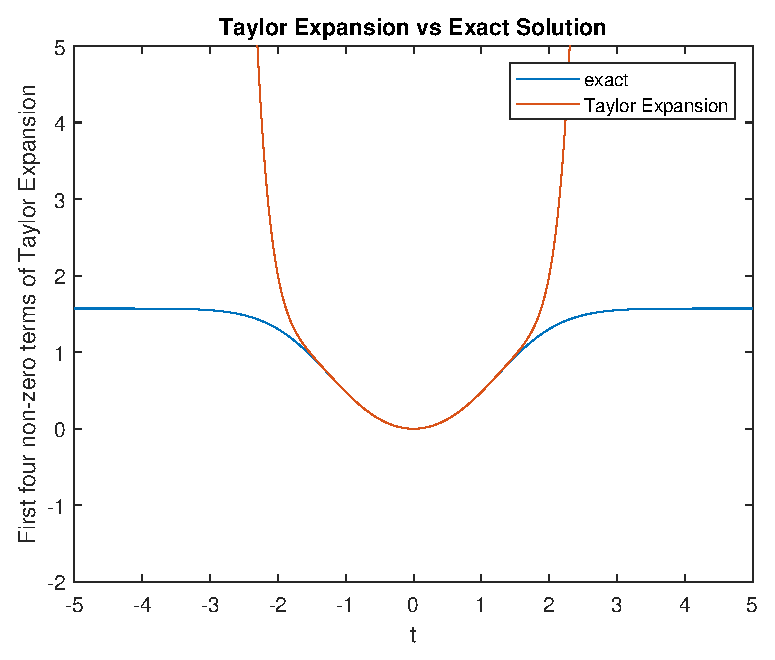
\includegraphics[scale=0.75]{TaylorSeries}
\end{figure}


Due to the difficulties of analytic integration, applying Picard iteration directly, as we did above, is often not feasible. However, by utilizing numerical integration techniques, Picard iteration provides us with a way to numerically approximate solutions to our IVP. Below is a MATLAB script that I wrote to perform Picard iteration utilizing numerical integration (trapazodial rule): 
\pagebreak
\section*{PicardIteration.m}
\lstinputlisting{PicardIteration.m}

In contrast to using Picard iteration with analytic integration, this method is extremely fast. For 35 iterations, this script takes only a few hundred milliseconds to run. Below we have plotted every fifth iteration against the exact solution to the above IVP:

\begin{figure}[ht]
    \centering
    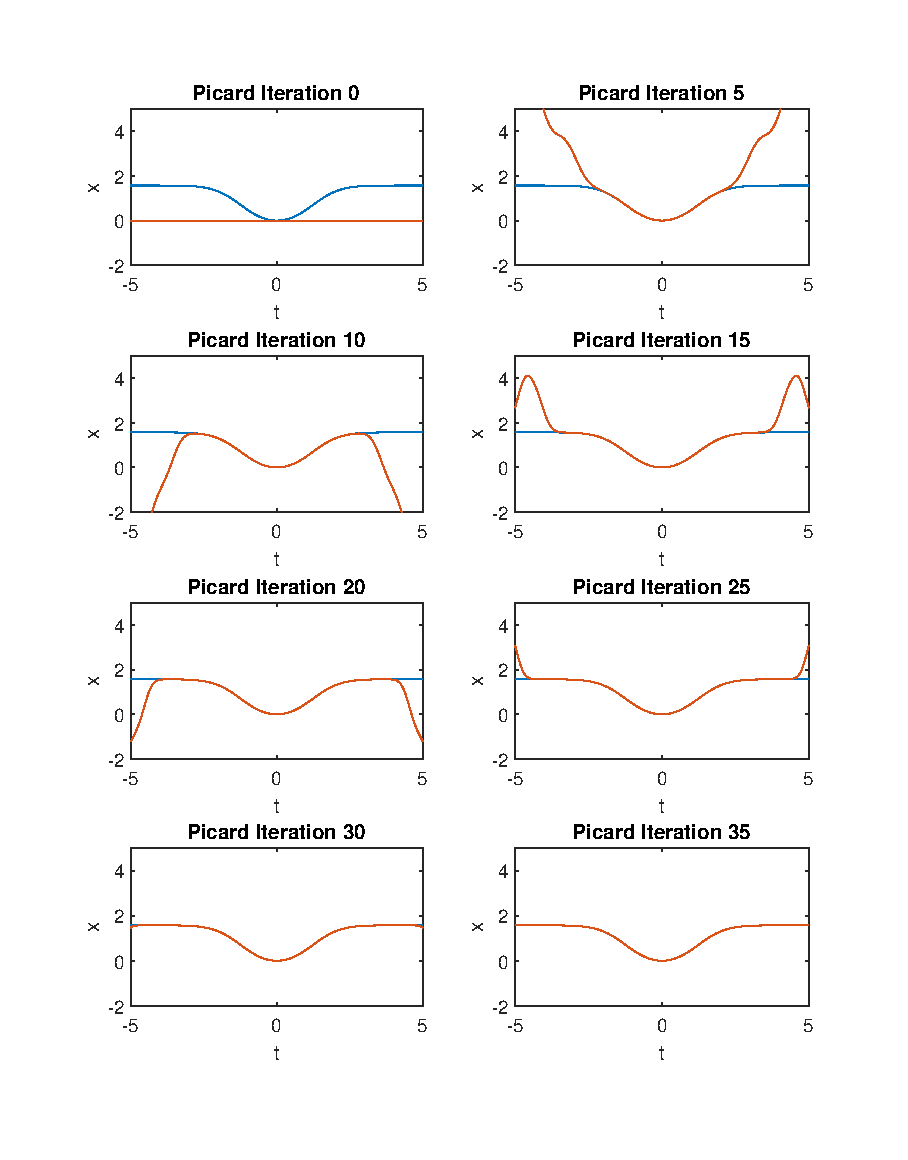
\includegraphics{PicardFig}
\end{figure}

\end{document}

